% \noman{This section should start with talking about the high level goals of our system.}
% The overall design of the OrchardScope system is shown in Figure~\ref{fig:architecture}.  
% The design decomposition is three tiers: the end nodes, the network, and the server-hosted, application-specific code. 
% We outline the details of each layer next. 
% The OrchardScope node supports a set of operations such as take images, run an image processing task, and communicate with nearby actuating device . The OrchardScope network is a wireless Bluetooth Low Energy (BLE) mesh network that uses a LTE-enabled gateway to route packets between the OrchardScope nodes and other networks. The application tier consist of precision agriculture applications that interacts with the network of OrchardScope nodes via its API.

OrchardScope design consists of three tiers: (1) The bottom-tier consists of densely deployed resource-constrained devices providing high spatial coverage. These devices are batteryless; they collect and transmit data intermittently. (2) The mid-tier comprise of devices capable of capturing and processing high-resolution data such as video streams. They are also responsible for powering up bottom-tier devices and reading data from them. (3) The top-tier is a cloud component connected to mid-tier through unreliable network, as is the case in most farm settings. This tier has excess storage and compute capability at the cost of high access latency.

\begin{figure}[t]
\centering
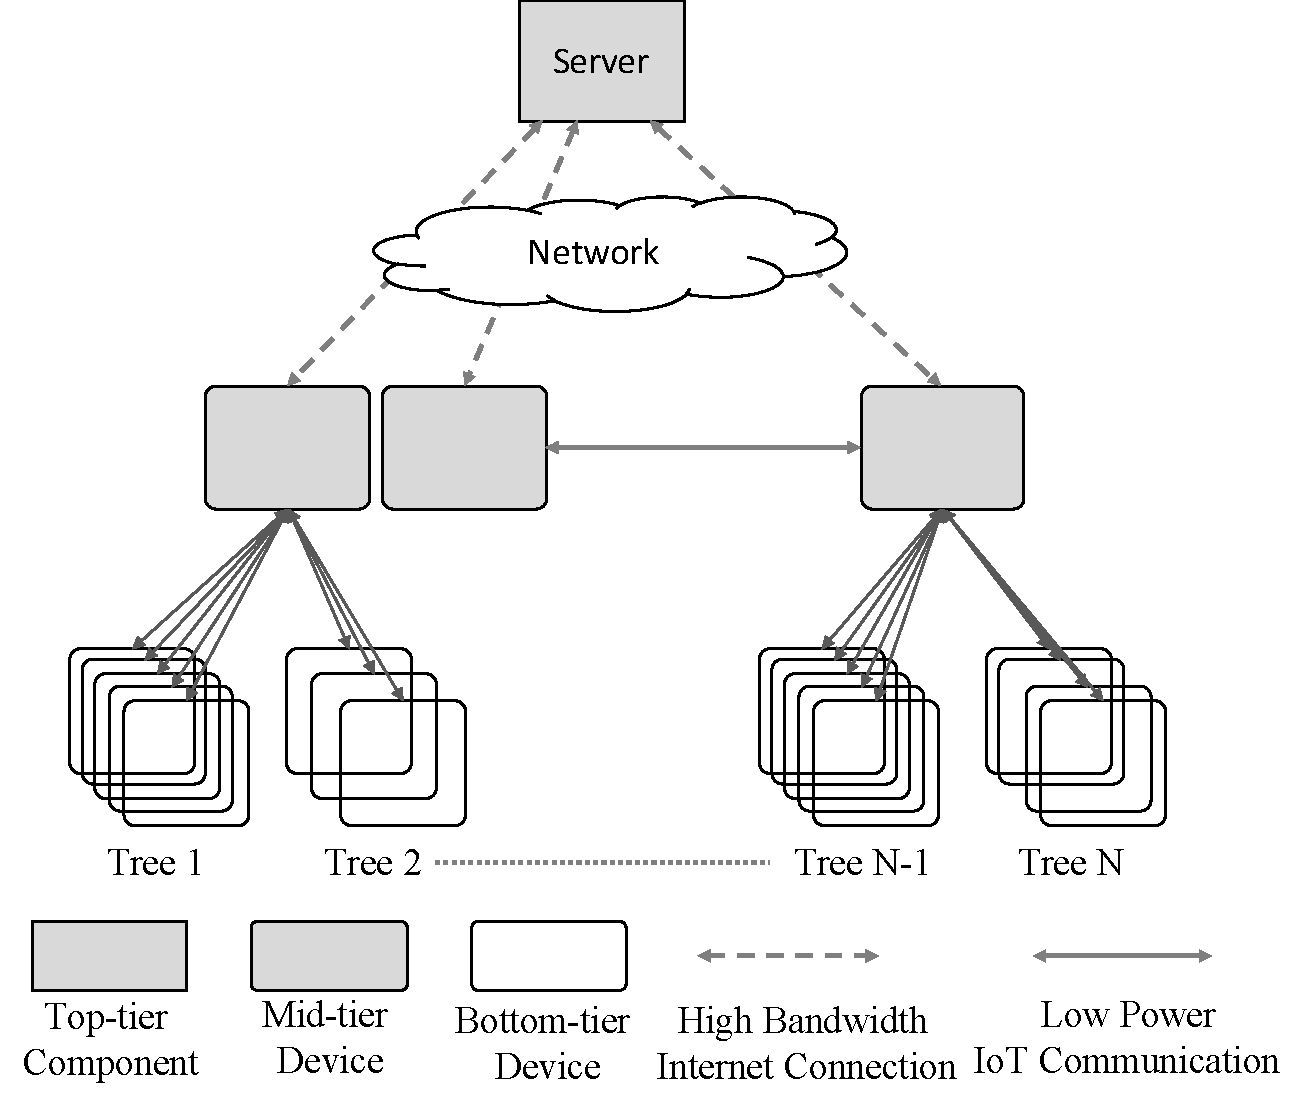
\includegraphics[width=0.4\textwidth]{./figures/arch_v2.pdf}
% \vspace{-0.4cm}
\caption{Three-tiered OrchardScope architecture}
% \vspace{-0.3cm}
\label{fig:architecture}
\end{figure}


\subsection{Bottom-Tier}
The bottom-tier consists of tiny, batteryless, and intermittently-powered devices that collect environmental variables such as humidity, temperature, pH value, soil moisture, etc. 
% Devices in bottom tier are only capable of data collection using tiny, batteryless, intermittently-powered devices.
\\\textbf{Device Placement:} 
The bottom-tier devices are densely deployed across the farm. For example, there may be multiple devices per tree that collect data from different parts, i.e. leaves, stem, top of canopy, soil, etc. 
The high spatial granularity can help in getting an insight into the existence of micro-climates, their effect on the yield, spread of diseases, the environmental conditions that lead to pest attacks or spread of fungi, etc.  
\\\textbf{Data Collection:} 
The primary purpose of these devices is to take a measurement of the environmental variable they are intended for. These devices take the measurement when they are powered by the power source and transmit the collected data to a reader, both located at the mid-tier device. The power source and the reader node may be same depending upon the technology. The nodes in this tier can only transmit data to mid-tier devices and cannot talk to each other. An existing technology for tiny, batteryless, and intermittently powered device is low power wireless sensing using Radio Frequency Identification (RFID). These tags cannot store energy and are triggered
using backscattering mechanism in radio frequency signals (RF). Also, nodes containing solar panels are intermittently powered through laser beam. 
\\\textbf{Challenges:} 
There are both hardware and software level challenges in this tier, some of those challenges are outlined below. 

\noindent
\textbf{Finding optimal reader-device distance:}
One of the main challenge is to calibrate the distance between these tiny devices and their readers for optimal data collection. Increasing the number of antennas on the reader potentially increases the communication range. Synchronizing various readers also add to spatial diversity, however implementing a timing service on resource constrained devices have its own challenges []. Another key challenge is to estimate how many devices can be accommodated by each reader given the device power requirement and time resolution constraints.   

\noindent
\textbf{Determining ideal power and duration:} An important challenge is to determine how much power and for how long is required for an accurate reading. It is important to strike the right balance as higher power levels for long duration may lead to time and energy waste, while low power for short duration may result in missing or erroneous data. 

\noindent
\textbf{Handling missing or erroneous data:}
 There is a possibility of missed or erroneous communication with any intermittently powered batteryless devices and a software capable of extracting knowledge from missed data needs to be explored. 


\subsection{Mid-Tier} 
The mid-tier consists of resourceful devices that collect data from bottom-tier, process and aggregate data from variety of sensors, make real-time actuation decisions, and forward the collected data to the top-tier. 

\noindent\textbf{Device Placement:} The mid-tier nodes are sparsely deployed across the farm. The placement of these devices depends upon the technology used in the bottom-tier, the resolution requirement of the video streams, and placement of actuating devices and their communication technology. For example, RFID-based bottom-tier nodes may require the mid-tier device to be at maximum of 100ft for reliable data collection, the camera resolution may dictate a mid-tier device for each block of trees, and actuation device communication technology may need the mid-tier node to be at maximum of 50ft. The mid-tier nodes placement is such that it satisfies all the constraints. 

\noindent\textbf{Mid-tier Services:}
Devices in mid-tier provide various services that are outlined below.
\\\textbf{1. Data Collection:} The mid-tier nodes power the densely deployed bottom-tier nodes in their vicinity and receive data from them. In addition, they also gather data from the high-resolution sensors that are directly interfaced with them, i.e. cameras, GPS, anemometer, pyranometer, etc. 
\\\textbf{2. Aggregation \& Inferencing:} The mid-tier nodes are responsible for aggregating data from different sources such as bottom-tier nodes and high-resolution sensors, in order to enable various precision agriculture applications. These applications use the aggregate data to make real-time inferences. For example, a disease detection application may combine high-resolution camera feed with the environmental variables such as temperature to detect the early signs of a disease, predict disease type, and estimate the extent of disease spread. The inference tasks are typically enabled by machine learning and computer vision techniques. To enable the data processing, aggregation, and inference tasks, mid-tier nodes require a processor that provides interfaces and have a capability to run ML/AI tasks, i.e. Jetson boards, Coral Edge TPU, BeagleBone AI, Arrow I.IMX8X, etc. 
% Aggregate data collected from bottom-tier devices and other mid-tier devices to make real-time inferences.
\\\textbf{3. Forwarding:} The mid-tier nodes are capable of horizontal as well as vertical communication in both directions. In vertical direction, they communicate with the bottom-tier to gather data from bottom-tier nodes and upload all the data aggregated at the mid-tier to the top-tier. In addition to the uplink communication to the top-tier, they also receive data and control instructions from the top-tier to enable precision agriculture applications. The link between the top-tier and mid-tier may be enabled by a high bandwidth communication technology such as WiFi, cellular, etc. The mid-tier nodes can also talk with each other to do data sharing, aggregation, and collaborative edge-computing tasks. For example, mid-tier devices may communicate to share the data about a tree that is partially covered by two devices or they may need to run a heavy ML/AI task across multiple devices. The link between the mid-tier devices will be enabled by low power IoT communication technologies such as BLE, IEEE 802.15.4, etc. 
\\\textbf{4. Actuation:} The mid-tier nodes communicate with the actuation devices to perform a task based on the real-time inferences. For example, a insecticide spraying application may require the mid-tier node to make a real-time inference on the population of insects that gathers after pheromone spray. Once the desired population is attracted, mid-tier node will actuate the insecticide spraying nozzle to kill all the insects. The actuation device may be directly interfaced with the processor through on-board interfaces such as USB, I2C, SPI, or connect wirelessly through a low power communication technology such as BLE, IEEE 802.15.4, etc. 
\\\textbf{Challenges:} When to power and collect data from bottom-tier nodes. Edge device and energy harvesting issues. Data aggregation or sensor fusion across various sensors etc. In all the discussion, motivate using agriculture use cases.
\begin{itemize}
    \item \textbf{Managing Bottom-tier Devices:} To enable high spatial resolution, bottom-tier nodes need to be deployed in large numbers in a way that does not require careful installation. In addition, these devices may move due to wind, rain, and irrigation water. The task of locating, powering, and reading data from these floating devices will present unique challenges. 
    \item \textbf{Energy Harvesting:} The grid power is typically not available in the farm and mid-tier devices will need to harvest energy for their operations from source such as solar PV, wind, etc. The energy harvested from these renewable resources is highly stochastic and dependent upon weather and shading from nearby trees. The mid-tier devices will encounter the challenge of predicting the expected energy into the future and schedule their operations based on the energy budget.  
    \item \textbf{Collaborative Edge Computation:} Some of the mid-tier services may need collaboration across devices. For example, a precision mapping application may need to combine/stitch data from multiple mid-tier devices or an analytics application may need to analyze temperature data at various points in the farm. These collaboration among devices raises challenges related to energy management, networking, and scheduling tasks. 
    \item \textbf{Data Aggregation:} The network connection with the top-tier can be unreliable, as in most farm settings. The network connectivity may be possible at only one or few of the devices in the mid-tier. This situation raises challenges related to data aggregation across nodes. 
\end{itemize}


% \fatima{You can replace "bottom-tier" sort of names with something relevant. Figure is only for reference. You can modify it in any way.}



\subsection{Top-tier}

The top tier is hosted in the cloud and provides the user an interface to deploy applications and access the data. The keys tasks we envision the user to perform are outlined. 

\noindent
\textbf{Top-tier Services: } The top-tier of OrchardScope provides various services that are outline below. 

\noindent
\textbf{1. Application Deployment:} The primary task of the user is to deploy applications ranging from generic tasks of gathering particular data at a desired granularity to specific applications such as monitoring insect traps. The applications combine both the data acquisition tasks as well as machine learning applications to decide on specific actions to take. 

\noindent
\textbf{2. Summary \& Overview:} The user will be able to access the summary of the collected data or results of deployed applications. For example, user may want to see the temperature at various parts of the tree or they may be interested in the number and types of insects captured by the trap. 

\noindent
\textbf{3. Raw Data Access:} The user, especially academic researchers, may be interested in accessing the raw data to either build new applications or retrain the existing ML applications using the most recent data. 

\noindent
\textbf{4. Data On-demand:} The application tier provides manual control to the academic researchers who desire the ability to control cameras and sensors to acquire data on-demand. 

\noindent
\textbf{Key Challenges:} We next outline the challenges faced in the design and development of the OrchardScope application tier. 
\begin{itemize}
    \item \textbf{Manual Control:} Providing manual user control while satisfying the requirements of the applications that are running on OrchardScope will be a challenging task. 
    \item \textbf{Edge Training:} There has been a lot of work on training ML models across distributed edge devices, cite[1,2]. However, training models on resource constrained solar-powered nodes will pose unique challenges. 
\end{itemize}


% \subsubsection{Performance Evaluation:} We will evaluate the system performance on the basis of average data rate achieved in the network, its packet reception rate, and the number of devices the network can support. 

% \subsection{Evaluation}
% This section outlines the proposal to perform evaluations for various aspects of the OrchardScope node. The first step would be to measure the actual power consumption of the devices under various operating conditions. The next step would be to measure the quality of DC power supply and its efficiency. The third step would be stress test the computaion engine of the node to see how much computation can it perform and how its power requirements change with the load. For the radio, we need to test the range and the data rate provided by the BLE enabled nodes. Finally, we should use solar performance modeling and forecasting to analyze the operation of the solar power supply for a typical year in various location inside United States. We plan to use Solar-TK, a black-box data-driven toolkit for solar performance modeling and forecasting for the task~\cite{bashir2019solar}. 



% \begin{figure}[t]
% \centering
% 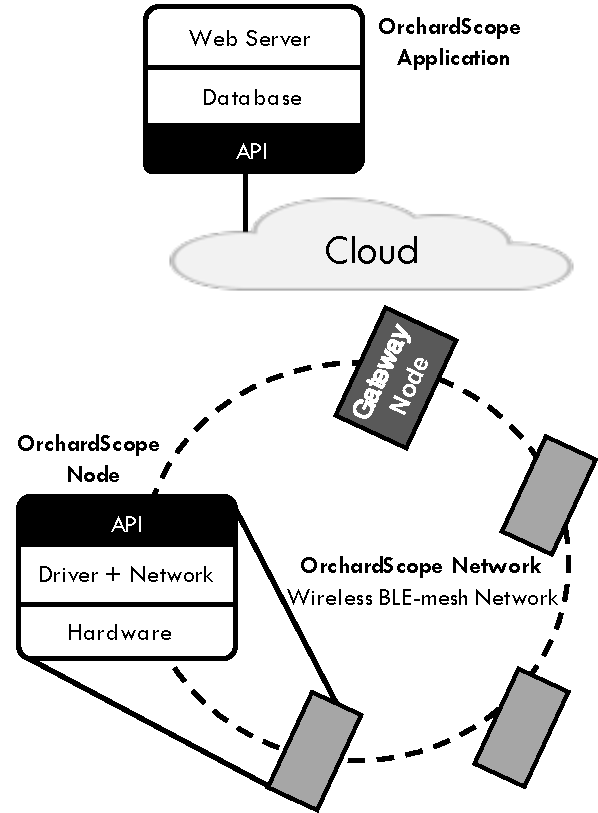
\includegraphics[width=0.4\textwidth]{./figures/architecture.pdf}
% % \vspace{-0.4cm}
% \caption{Three tier OrchardScope system.}
% % \vspace{-0.3cm}
% \label{fig:architecture}
% \end{figure}

% In the following sections, we present the design and implementation of each tier of the OrchardScope system.  At the node level, we discuss the various trade offs present in the hardware design, and present a narrow interface to access the hardware. Equally important, we consider physical design issues such as form factor and weather-proofing, which must be addressed for a deployment in an outdoor setting to be practical.  The result is the OrchardScope node:  a small form-factor device with sensing, control, and networking integrated into one package. 

% A set of disconnected monitoring devices is much less interesting than real-time data. The current wireless sensor network applications in agriculture monitoring typically use standalone designs that target one specific application, have a small LCD, a serial port, or other wired ports connecting instruments to data loggers. 
% A key motivation of our work is to allow the quick deployment and instrumentation of a large numbers of monitoring devices and enable continuous real-time access. Requiring connectivity over USB, serial, Ethernet,  or other wired channel would not be practical.  

% Finally, application specific code is placed in the cloud that is connected to the OrchardScope nodes network. Applications use the node API as exported over the network. Typically, a server daemon populates a database that is accessed by a variety of web applications, but direct access to OrchardScope using REST API is available too. We present an apple cluster thinning application which allows researchers to monitor the apple cluster over time, deploy computer vision algorithms to determine the cluster sizes, and perform the computation to determine the amount of thinning spray needed. A key architectural separation is that applications are developed independently from the network used. 


% \subsection{OrchardScope Node}

% The OrchardScope node consists of four primary components: sensors, power supply, processing unit, and a radio for OrchardScope network
% % , as shown in Figure~\ref{fig:node}
% . We next describe the choice of OrchardScope node components and how each satisfies the high-level goals of OrchardScope system. 

% % The sensor component is user-configurable where user can select which sensors are attached to the device, i.e. camera, temperature, moist, and humidity. The data from the sensing components is received by the computational engine, which processes the data using sensor-specific pre-processing techniques. The computational engine is also responsible for running the user-specified machine learning or computer vision models on the data. The power source components harvests solar energy and converts it to the appropriate DC levels required by the various components in the system. Finally, the radio is used to communicate with other devices in the network. While most of the devices in the network will have the aforementioned four components, the gateway devices in the network will have additional radios that will allow internet connectivity. 

% % There are several design choices for each component, each with its own advantages and disadvantages.  Design  decisions  for  the  different  components  of OrchardScope are not independent.  For example, a particular choice of internet connectivity enabling technology  will dictate how much computational power we have at the edge. We find that there are only a few internally consistent combinations, each appropriate for a distinct class of applications. To fully explore the available design space we plan to build two types of nodes, one for monitoring in-door spaces such as greenhouses with grid connection and WiFi connectivity available, and the other for the outdoor spaces without any power source and internet connectivity.  We plan to compare the two designs and evaluate their effectiveness for our application in future.

% % \begin{figure*}[t]
% % 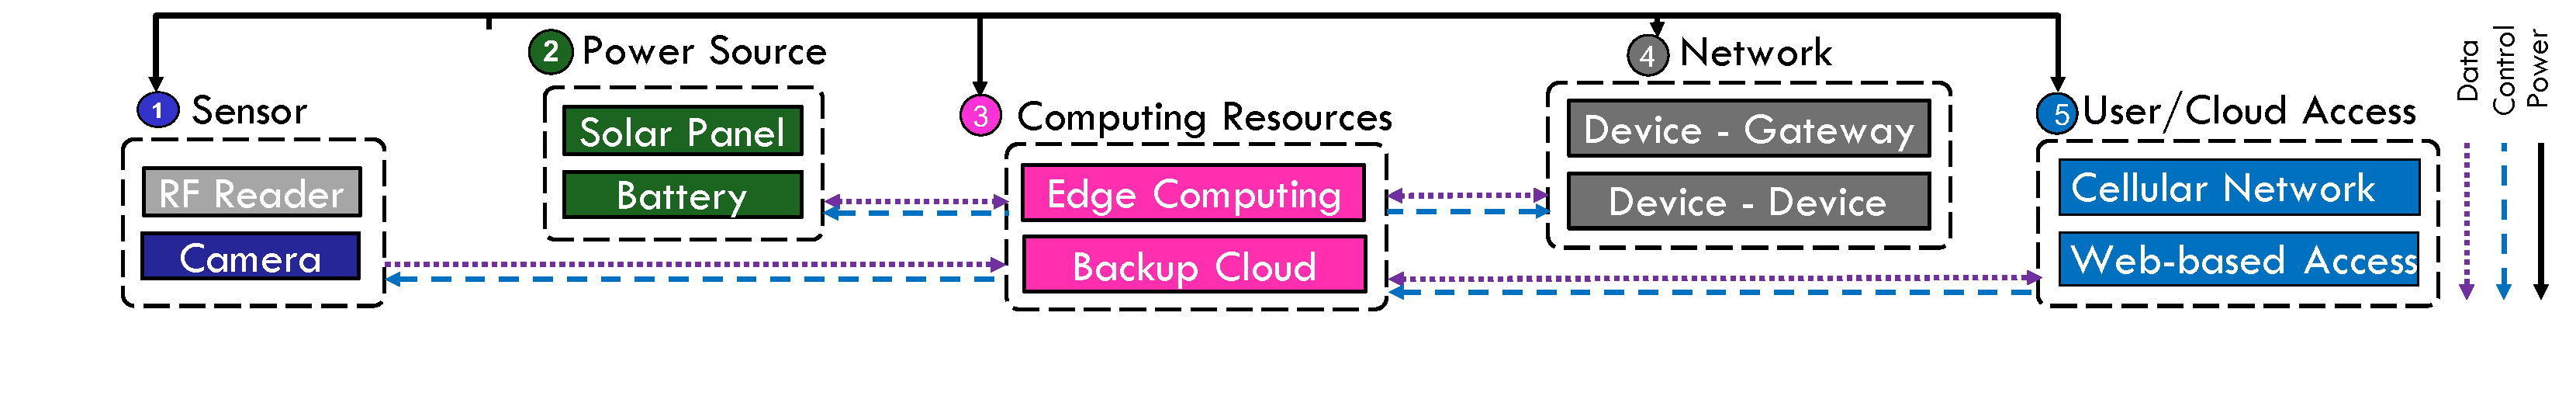
\includegraphics[width=\textwidth]{./figures/node.pdf}
% % % \vspace{-0.4cm}
% % \caption{OrchardScope consists  of  five  primary  components:   sensors, DC power supply, computational engine, a radio for OrchardScope network, and an optional radio for internet connectivity.}
% % % \vspace{-0.3cm}
% % \label{fig:node}
% % \end{figure*}

% \noindent
% \textbf{A. Sensors:}
% \label{sec: sensors}
% Two types of sensors are connected to the OrchardScope node: cameras directly connected to the node and environmental sensors interfaced using RFID reader.

% % There are multiple sensors that can be used to measure various aspects of agriculture, i.e. humidity, temperature, soil moist level, and wind speed sensors. However, while designing the OrchardScope, we are primarily interested in deploying a camera to enable computer vision based precision agriculture applications. We evaluate the difference and trade-offs between various architecture to provide visual coverage of the farm based on the extent of coverage provided and cost incurred. 

% \noindent
% \textit{\textbf{Cameras.}}
% The goal of the cameras is to take high resolution images of the different entities inside the farm, i.e. tree leaves, leaf stems,  fruits, insect traps, and ground under the trees. To meet these requirements, we use a variable focal length high resolution camera with pan-tilt-zoom (PTZ) capabilities. The focal length of the camera is chosen such that it is able to take the image at the required resolution (i.e. 1080p) of the desired object (i.e. leaves 5inx5in) at a distance (i.e. 30ft). Simultaneously, it should have a wide view to capture low resolution wide images for the applications that do not need high resolution, i.e. counting dropped fruits on the ground. 

% % Focus on design as drones have already been discussed in motivation section.

% % points
% % Drones are not good. 
% % Static cameras either do not provide high resolution or very high resolution cameras are very expensive. 
% % The solution is the variable focal length high resolution camera. 
% % It provides high resolution images of the farm at various scales. 

% % Drones are the most commonly visual sensing equipment used for mapping the fields and farms in various precision agriculture applications. However, drones are not suitable for applications where you need visual data at high temporal resolution, require high resolution images of small parts of the farm i.e. tree leaves, and have 

% % They are suitable for applications where the temporal resolution of visual data captured is low. However, if the images are required more frequently, the drones may not be a suitable option as it would not give the drones enough time to recharge the batteries. It would be an option to increase the size of drone fleet, but it would incur additional costs and operating a large fleet would be complex. In addition, the drones may require FAA approval for their operation.  

% % Most of the precision agriculture application that we consider need images of tree leaves and fruits, i.e. apples in case of an apple orchard. Given this scenario, one option was to install a low resolution cameras on the tree branches and very near to the subject that needs to be captured. This option allows us to use low-cost, low resolution cameras and still get high enough resolution required for our tasks. However, installing devices on tree branches will require careful human labour-intensive installation and maintenance. In addition, the devices may get damage during the spraying or other invasive tasks on the tree. 

% % The other end of the spectrum is to install a single, high resolution camera with telephoto lens on top of a pole in the middle of the farm. In this case, the camera is capable of taking wide pictures of the farm and has the ability to zoom into specific parts of the tree to take pictures of apple clusters and leaves, if needed. This design choice offers easy installation and maintenance. However, the key problem with this choice is the cost and the single point of failure. The cost per unit area of very high resolution cameras ends up being much higher than any of the other options we consider. In addition, installing a very expensive single camera is not practical in the sense that the data will not be collected if it goes down and also the cost to replace it would mean building almost everything from scratch again.  

% % A moderate option would be to install mid-resolution cameras distributed throughout the park that monitor only a couple of trees that are nearby. This option lies between the option 2 and option 3 in terms of cost and complexity of installation and maintenance. We have decided on using a static focal length camera without the zoom capability, as we determined that the cameras with the programmable zoom capability were significantly expensive than those of static focal length. Therefore, instead of zooming into different places, we plan to take images with a fixed zoom and adjust the distortion in the software. This setup also requires a pan-tilt assembly that allows the camera to capture multiple trees. Also, the devices containing cameras would connect with each other using a mesh network and be able to share the data they gather. 

% % The choice of camera is dictated by three factors: the size of the object to be captured, the distance of the object from the camera and the required resolution for the image. A typical apple cluster is 12in x 12in, it is at a 15-20ft distance from the camera, and we would like to capture the image at 1080p atleast. Given these specifications, we can use the arc length formula to compute the field of view for the camera. If the radius is r, and the internal angle is $\theta$, the arc length is L is given by $r\times \theta$. We can compute the internal angle required from this equation, which comes out to be $\sim 5.4^o$ for a 1080p resolution camera or $~\sim 21.6^o$ for a 4K camera. The relationship between the field of view (FOV) and the focal length is given by the following equation. 

% % \[FOV = 2 \times arctan (x / (2 f)) \]

% % Here, f is the focal length and the x is the diagnol of the area that we are trying to capture. Using this formula, the focal length required for the 4K camera comes out to be around 113mm. 

% \noindent
% \textbf{\textit{Passive RFID Sensors for Environmental Variables.}} Our system monitors the different environmental variables, i.e. temperature, humidity, using low-cost RFID-based sensors that are densely deployed across the farm. The sensors are passive and need to be powered by an RFID reader when the measurement is to be taken. The RFID reader integrates with the OrchardScope node and is controlled by the OrchardScope application to gather data at the desired time granularity. The details on the design of the sensors, their deployment, and data collection mechanism are outside the scope of this paper. 

% % \fatima{Have a single subsection on cameras and also talk about RFID tags on leaves and how you need a reader at the edge too.}

% \noindent
% \textbf{B. Power Supply:}
% The OrchardScope node will typically be deployed in the wild, where the power grid is not available. Our design uses solar power coupled with a battery-backup to power the OrchardScope node. The size of the solar panels and batteries is dictated by the power requirement of different OrchardNode components, the resource requirements of OrchardScope applications, and the days of autonomy desired for places which observe extreme weather conditions such as snow storms. Therefore, the sizing of solar + battery backup is an implementation-specific and we use an approach outlined in [cite] to determine the actual size of panels and batteries. 

% The different components of the OrchardScope node may have different voltage requirements, i.e. embedded devices typically require 5VDC while cameras may need 12-24VDC. Therefore, we use DC-DC converters to provide 5V and 24V, in addition to the 12V battery outlet, as all of the OrchardScope node components operate on one of these voltages. 

% % In such scenarios, wireless sensor networks rely on either using batteries or harvesting energy available in the environment. The batteries are not ideal for our energy-intensive devices as we require data collection and processing at high temporal resolution. Solar panels coupled with a battery backup for night time operation are the most popular choice now a days. We next present the design of our solar + battery backup. 

% % \textbf{Solar + Battery System Design:} The sizing of solar panels and batteries for specific energy needs is a well-studied problem. The first step in this process is to estimate the net energy requirement for the system. In OrchardScope, the major components that consume energy are the Jetson Nano board, camera pan-tilt assembly, camera, and radio. The power requirements and the daily energy requirement for each of the components is listed in the Table~\ref{tab:energy_requirement}.

% % \begin{table}[]
% % \begin{tabular}{|l|l|l|}
% % \hline
% % \textbf{Component} & \textbf{Power (W)} & \textbf{Energy (Wh/day)} \\ \hline
% % Jetson Nano        & 10                 & 60 @ 20minutes/hour                \\ \hline
% % Camera             & \textless 5        & 30 @ 20minutes/hour                \\ \hline
% % Pan-tilt assembly  & \textless 5        & 30 @ 20 minutes/hour               \\ \hline
% % Radio              & negligible         & negligible                         \\ \hline
% % Misc               & variable           & 30                                 \\ \hline
% % Total              & $\sim$35           & 150                                \\ \hline
% % \end{tabular}
% % \caption{Power requirement and energy consumption of various components}
% % \label{tab:energy_requirement}
% % \end{table}

% % The average energy requirement for the whole system is $\sim$150Wh. However, solar power is highly dependent on weather and in some places, i.e. northeast USA, there may not be any solar generation following a snow event. 
% % Therefore, we would like to have some backup energy stored in the battery for the days when there is no generation. We pick 3 days of autonomy for our system, which means that the total energy to be stored in the battery backup should be $(1+3) days\times 150Wh/day = 600Wh$. The size of the battery to store 600Wh at 12V should be 50Ah. Assuming 50\% depth of discharge, the lowest state of charge allowed, the battery size should be 100Ah in order to ensure longer life for the battery. The next task is to decide on the size of the solar panel such that the energy generated in a day should be 600Wh. We can assume the average day light hours to be 8hrs for most of the places in the United States. This setup means that the size of the solar panel should be $600Wh/8h = 75W$. However, the solar panel would not always produce 75W for all 8hrs of the day. Therefore, we need to pick a slightly bigger panel size of $\sim$100W. 

% % We have sized the solar panel and the battery backup for the energy requirement that we have chosen. However, this systematic approach can be used for sizing the solar panel and the battery backup for any energy requirements. 

% % \textbf{DC Power Supply Design:} We design our power supply as online backup where solar panel charges the battery and all the components are connected to the battery. This ensures that the short fluctuations in the solar power do not effect the power quality of the DC power supply. While the battery voltage is 12V, the different system components may not operate at the 12V, i.e. Jetson Nano requires 5V power supply while pan-tilt assemply needs a 12V power supply. Therefore, we design our system to provide all the different voltage levels required by the different components, which in this case are 12V and 5V. We can get the 12V directly from the battery, but a DC-DC converter is required to step-down the voltage level from 12V to 5V. The design of an efficient DC-DC converter is outside the scope of this paper and we simply use a DC-DC converter IC for this task. 

% \noindent
% \textbf{C. Processing Unit:}
% OrchardScope node uses Jetson Nano~\cite{jetson-nano} as its main processing unit because it offers a low-cost solution to run multiple machine learning applications in parallel while enabling easy interface of variety of sensors, i.e. cameras through CSI or ethernet interface, RFID reader using xyz. 
% The small size and low-power requirement make it suitable for in-the-wild and low energy applications. The computing power at the edge provided by Jetson nano allow us to enable applications that require real-time response even in the presence of low/intermitten Internet connectivity. 

% % There are four key tasks that will be performed at the OrchardScope node. The first task is the collection of data from the sensors. The second task is to clean the data and prepare it for various applications. The third task is to perform application specific tasks on data i.e. running a computer vision or image processing model to determine the attack of a pest. The final task is to make the findings available to the end user. 

% % One of the key goals of OrchardScope is to provide real-time feedback required for some precision agriculture applications. 



% % The first task of data collection needs to happen at the end device, while the other tasks can be done at the edge device or the data can be sent to the cloud where all processing is done. The cloud option is attractive as it provides infinite capacity and is cost-effective due to intense competition among cloud providers. However, it has two major drawbacks. The first drawback is that sending all the data to the cloud and back would generate a lot of data traffic. This is generally not a problem for WiFi networks, but it would be incur very high costs for scenarios where internet connectivity to the farm is established only using LTE technology. It would also incur high network and storage costs from the cloud provider. In addition to this, the second drawback is that the cloud-based computation will not be able to support real-time applications that researchers or farmers may want to deploy. 

% % Considering our choice of network and the cost of a cloud-based option, we have decided to put enough processing at the edge to enable real-time applications and use the cloud to only provide the user interface. We use Jetson Nano as the primary processing unit as it offers the general purpose IO ports (GPIO) for sensor interfacing as well as enables various machine learning model deployments. It is a small, powerful computer that lets you run multiple neural networks in parallel for applications like image classification, object detection, segmentation, and speech processing. Another attractive feature for the Jetson Nano is its very low power consumption of around 10W at its maximum use. 

% % In our setup, the Jetson Nano is responsible for collecting data from the sensors using different interfaces, i.e. USB for camera, I2C to control pan-tilt assembly. It then processes the collected images for different applications i.e. concatenates the smaller images at high resolution to generate bigger images that may be required for some other applications. Finally, it runs the user-specified machine learning tasks on the collected visual data, i.e. using computer vision to determine the size of the apples in the clusters. The final task of providing user access is done through the cloud as this OrchardScope edge network may not be available all the times. 

% \noindent
% \textbf{D. Radio:}
% The next key component is the radio that we use for the communication between the devices and the device's connectivity to the internet. OrchardScope node uses Bluetooth Low Energy (BLE) radio to communicate with its peers due to its low cost, low power, and inherent support for mesh networking. BLE 5.0 offers data rates upto 5Mbps, which enable collaborative edge applications. OrchardScope uses a gateway node that gathers data from the orchardscope nodes to send to the cloud and also receive application code from the cloud that is deployed across the network. We use cellular network to provide the edge-cloud connectivity due to its ubiquity and high data rate. A third radio on the gateway device is that enables high bandwidth link between the gateway and the moving vehicle that collects raw data. \noman{needs discussion.}
% % Both communication tasks present different challenges and we decided to use different communication technologies for each, the choice and properties for each network are described next. 

% % \noindent
% % \textit{\textbf{OrchardScope Network.}} This is the network that exists between the OrchardScope nodes deployed at the edge. The key requirement for the communication technology for this part of the network was that it is low cost, low power, and offers support for mesh networking. The WiFi was an option, but its relatively higher cost and high power requirement made it unsuitable for the task. 802.15.4 based protocols/technologies i.e. ZigBee offered low power and low cost, but the maximum data rate of $\sim$250kbps was very low for some of the collaborative edge applications we envisioned. Therefore, we decided to use the Bluetooth Low Energy (BLE) mesh network as it provides inherent support for mesh networks, is low cost, low power, and its 5.0 specifications support data rates upto 2Mbps. We have decided to use nRF52 BLE development kit for our prototype, which supports BLE mesh network. 

% % \noindent
% % \textit{\textbf{OrchardScope Cloud Connectivity.}} The second aspect of the network design was to provide cloud connectivity to the devices and allow user to access the data. The devices use BLE mesh network to communicate with each other, we decided to use LTE to connect the devices to the internet. One option was to equip each device with LTE, but this would have increased the cost of each device. The other extreme was to have a single gateway device in the network that gathers data from all the devices and connects to the internet. We decided to use a moderate scheme where gateway devices are spread throughout the network to provide redundancy for the connectivity and also enable the high data traffic that may be needed to upload high resolution video data to the cloud. We plan to investigates the LTE capability and which specific module is to be used. 

% \noindent
% \textbf{E. Node Software:} 
% The OrchardScope node needs to implement some functionality in the software to enable some of the applications. The first key task is the acquisition of visual and environmental data by controlling camera and RFID reader, respectively. The camera control strategy decides on which object to capture, when to capture, and the desired resolution of the object of interest. Similarly, RFID reader control decides on which passive sensors to power, the time duration and strength of power, and how often the data should be collected. The next task is to process the collected data and prepare it for OrchardScope applications as well as sharing with the end user, i.e. concatenating partial images collected from different cameras. The third task is to run the machine learning and computer vision models that the user may have deployed as a part of OrchardScope application. Lastly, the node needs to manage its energy budget by forecasting solar power and estimating the energy requirement of different tasks, i.e data acquisition and running ML models. 


% % \noindent
% % \textit{\textbf{Camera Control.}} As discussed in Section~\ref{sec: sensors}, we have decided to use a mid-resolution camera mounted on a pan-tilt assembly that covers multiple trees. In order to enable that, we needed to design a camera control strategy where we decide on how we move camera to capture all the different parts of the trees under observation. There are two important factors that govern this decision: the distance of the tree under observation from the camera and the minimum resolution of the pan-tilt assembly. In our example deployment case, the distance between the camera and the tree ranges from 15ft-20ft. The minimum resolution provided by the pan-tilt assembly is $0.29^o$. A movement of $0.29^o$ by the pan-tilt assembly will shift a distance of 0.91in and 1.21in at 15ft and 20ft, respectively. The distance is approximately computed by the following formula. 

% % \[ arc\ length = radius \times central\ angle \]

% % This resolution is high enough to capture the smallest parts of the tree. However, as it is evident, the distance moved by a fixed degree movement by the assembly depends upon the distance of the tree from the camera. Therefore, we will need to adjust the angle moved in order to get the consistent coverage of the trees under observation. In our current implementation, our camera control algorithm simply divides the area under observation into a grid where it moves along the rows from left-right (for odd rows) and right-left (for even rows). This approach is simplistic but has two key drawbacks. First, we may be interested in capture only a particular part of the trees and we would need to reconstruct the whole image from these small parts and then find the desired image from the bigger picture. Secondly, the individual pictures along may not capture the desired object fully, i.e. an apple cluster that we want to capture may be divided in two cells. This would also require generating a bigger picture from the parts and locating apple clusters. However, this reconstruction will incur some losses and the desired object may be deformed. 

% % We are considering using computer vision techniques to identify where the images need to be taken. For example, in case of capturing apple clusters, the camera will scan the apple tree and the video stream would be processed by a computer vision model which will save the image only if it captures the object under consideration. However, this requires pre-training of the models to detect the desired objects. The acquisition of data for the training and training may not be very straightforward. 

% % \noindent
% % \textit{\textbf{Image Concatenation.}}
% % The mid-reolution camera only captures a 1080p images of a 5in$\times$5in image. However, for some of the applications, the researcher may require a bigger image and the smaller images may need to be concatenated. We currently implement a very simple image concatenation technique which uses Python Pillow library to stack images together. However, this assumes that all the images do not overlap and the do not have distortion. These assumption may not hold true in practice as imprecise movement of pan-tilt assembly would result in some overlap or some parts of the images missing. Also, the pictures will be taken at different distances from the camera, which means the size of the images and the angle at which the image is taken will be different. There is a need for a better concatenation techniques that considers these problems and generated better concatenation. 

% % \noindent
% % \textit{\textbf{Weather Forecasting.}}
% % We plan to leverage a probabilistic forecasting approach developed by one of the authors. The paper outlining the approach is under-review and we are not providing the details of the approach here to comply with the condition of double blind review process.

% % \noindent
% % \textit{\textbf{Computer Vision Models.}} The OrchardScope node will also enable the user to run computer vision and other machine learning models. We are working on figuring out on how to expose this functionality to the end user and how the pipeline should look like. 

% % \fatima{We don't need too much details in all of these subsections. Focus on key points that are hardware-agnostic. Try to be as general as possible by highlighting key challenges and solution. In terms of naming specific technologies, use them only when necessary, otherwise it does not feel like a generalized architecture.}

% \noindent
% \textbf{Key Challenges:} We next outline the key challenges in the design and development of the OrchardScope node. 
% \begin{itemize}
%     \item \textbf{Camera control:} OrchardScope uses variable zoom cameras at high focal length to capture the images at high resolution. The high resolution and under-wind operation poses a challenge to taking high quality images. 
%     \item \textbf{Object Identification:} OrchardScope applications may require monitoring certain part of the trees or other objects, i.e. insect traps periodically. The task of initially locating the object and revisiting at the same angle poses a significant challenge. 
%     \item \textbf{Weather-aware Operation:} Prior precision agriculture systems, such as FarmBeats~\cite{vasisht2017farmbeats}, use solar forecasting to duty-cycle their sensor modules. However, combined scheduling of ML tasks at the edge, data acquisition from sensors, and cloud connectivity under unpredictable weather poses unique challenges. 
% \end{itemize}

% \subsection{OrchardScope Network}
% We have decided on using the BLE-mesh network for the OrchardScope system. We still need to figure out how that system would look like. However, the discussion about the network will revolve around the BLE mesh network, the gateway device, and the performance evaluation. 
% \noman{Not entirely clear on what goes in this section, will revisit later. }

% \noindent
% \textbf{A. Node-node:} In this section, we will talk about the BLE-mesh specifications and how it will be deployed on the Jetson nano board. 

% \noindent
% \textbf{B. Node-cloud:} In this section, we will talk about the LTE-enabled gateway device that will gather data from all the devices in the mesh network and send this data to the cloud. 

% \noindent
% \textbf{C. Node-Vehicle:} The cellular network is not ideal to transfer large data collected in the form of high resolution images. To collect the raw data from the edge-devices, we use the tractors and robotic vehicles that travel the farm on regular basis. 

% \noindent
% \textbf{Key Challenges:} We next outline the challenges faced in the design and development of the OrchardScope network. 
% \begin{itemize}
%     \item 123
%     \item ABC
%     \item XYZ 
% \end{itemize}



